\documentclass[logo=images/logo.png]{tehranReport}
\usepackage{arydshln}
\usepackage[inline]{enumitem}
\usepackage{verbatim}
\usepackage{amsmath}
\usepackage{amssymb}
\usepackage{mathtools}
\usepackage[dvipsnames,table]{xcolor}
\usepackage{listings}
\usepackage{float}
\usepackage{geometry}
\usepackage{hyperref}
\usepackage{xepersian}
\usepackage{footnote}
\usepackage{pifont}


\settextfont{XB Niloofar}

\title{پروژه‌ی ۱ - گزارش}
\author{\href{mailto:ranjbar.ali@ut.ac.ir?subject=[OS\%20S99 L1]\%20}{علی رنجبر}}
\authorPosition{دانشجوی کهاد مهندسی کامپیوتر~~نرم افزار}
\studentNumber{810097029}

\secondMember{{\href{mailto:ranjbar.ali@ut.ac.ir?subject=[OS\%20S99 L1]\%20}{عضو دوم}}}
\secondMemberPosition{دانشجوی کهاد مهندسی کامپیوتر~~نرم افزار}
\secondMemberStudentNumber{810097029}

\thirdMember{{\href{mailto:ranjbar.ali@ut.ac.ir?subject=[OS\%20S99 L1]\%20}{عضو سوم}}}
\thirdMemberPosition{دانشجوی کهاد مهندسی کامپیوتر~~نرم افزار}
\thirdMemberStudentNumber{810097029}

\university{دانشگاه تهران}
\college{پردیس دانشکده‌های فنی\\دانشکدهٔ مهندسی برق و کامپیوتر}
\studentNumber{810097029}
\course{آزمایشگاه سیستم عامل}
\supervisor{دکتر کارگهی}
\graphicspath{{./images/}}

\tolerance=5000
\renewcommand{\thesection}{\arabic{section}}
\renewcommand{\thesubsection}{\arabic{subsection}}

\begin{document}
	\maketitlepage
	\section*{آشنایی با سیستم عامل \lr{xv6}}
\begin{enumerate}
	\item 
	\textbf{معماری سیستم عامل \lr{xv6}: }
	\lr{xv6} 
	دوباره پیاده‌سازی سیستم عامل 
	Unix 
	که توسط دنیس ریچی
	\LTRfootnote{Dennis Ritchie} 
	و کن تامسون 
	\LTRfootnote{Ken Thompson} 
	معرفی شد، است. این سیستم عامل با معماری یکپارچه 
	\LTRfootnote{Monolithic} 
	طراحی شده کل سیستم عامل در فضای هسته 
	\LTRfootnote{Kernel space} 
	اجرا می‌شود و یک رابط برای اجرای برنامه‌های کاربر ارائه می‌دهد.
\end{enumerate}
	\section*{مراحل اجرا و بوت}
\begin{itemize}
	\item [2] 
	\textbf{گروه \lr{basic headers}}: 
	این گروه شامل فایل‌های سرایند اساسی است. مانند 
	\lr{\lstinline|types.h|} 
	که شامل تعاریف انواع داده‌ای مورد استفاده در کد برنامه است یا 
	\lr{\lstinline|param.h|} 
	که شامل پارامترهای اولیه (مانند انواع محدودیت‌ها: محدودیت تعداد پردازه‌ها، محدودیت تعداد CPUها و ...، اندازه‌ی بلوک‌های مختلف و ...) برای سیستم عامل است.
	
	\textbf{گروه \lr{entering xv6}}: 
	این گروه شامل فایل اصلی 
	\LTRfootnote{main} 
	برنامه و دو فایل اسمبلی دیگر برای شروع به کار سیستم عامل است. شروع کد سیستم عامل در فایل‌های این گروه قرار دارد.
	
	\textbf{گروه \lr{locks}}: 
	همان‌طور که از اسم این گروه معلوم است، پیاده سازی مربوط به قفل‌ها در این گروه قرار دارد.
	
	\textbf{گروه \lr{processes}}: 
	تمام پیاده سازی‌های مربوط به پردازه‌ها اعم از حافظه‌ی مجازی، جدول صفحه
	\LTRfootnote{page table}، 
	مدیریت حافظه‌ی فیزیکی، جابجا شدن بین پردازه‌ها و ... در این گروه قرار دارند.
	
	\textbf{گروه \lr{system calls}}: 
	در این گروه توابعی برای راحتی کار با فراخوانی‌های سیستمی نوشته شده است. همچنین رسیدگی به وقفه‌ها نیز در این گروه انجام می‌شود.
	
	\textbf{گروه \lr{file system}}: 
	همان‌طور که می‌دانیم، 
	\lr{xv6} 
	در معماری خود رابطی بسیار کاربردی به اسم فایل دارد که سطح انتزاع 
	\LTRfootnote{Abstraction level}
	خوبی برای عملیات 
	\lr{I/O} 
	فراهم می‌کند. پیاده سازی‌های مربوط به این رابط در این گروه قرار دارند.
	
	\textbf{گروه \lr{pipes}}: 
	پیاده سازی ویژگی پایپ (روشی برای ورودی و خروجی)
	
	\textbf{گروه \lr{string operations}}: 
	در این گروه توابعی مفید برای کار با رشته‌ها تعریف شده‌اند.
	
	\textbf{گروه \lr{low-level hardware}}: 
	پیاده سازی‌های سطح پایین برای دسترسی به سخت افزار در این گروه قرار دارند. (ارتباط با سریال، پردازش‌های چند پردازه‌ای و ...)
	
	\textbf{گروه \lr{user-level}}: 
	برنامه‌های کاربردی سطح کاربر در این گروه قرار دارند. (مانند برنامه پوسته 
	\LTRfootnote{Shell})
	
	\textbf{گروه \lr{bootloader}}: 
	برنامه‌ی 
	\lr{boot loader} 
	برای شروع به کار اولیه (هسته‌ی) سیستم عامل (کپی کردن سیستم عامل در حافظه)
	
	\textbf{گروه \lr{link}}: 
	اسکریپتی برای لینکر هسته
	
	\textbf{در سیستم‌عامل لینوکس} 
	فایل‌های هسته‌ی سیستم عامل در پوشه‌ی 
	\lr{kernel}، 
	فایل‌های سرایند در پوشه‌ی 
	\lr{include} 
	و فایل‌سیستم در پوشه‌ی 
	\lr{fs} 
	قرار دارند.
	\item [3]
	خروجی دستور 
	\lr{\lstinline|make -n|}: 
	\begin{latin}
		\lstinputlisting[language=bash,caption=make -n,label=maken]{maken.log}
	\end{latin}
	با توجه به 
	\ref{maken} 
	بعد اجرای خط ۱ فایل‌های باینری ساخته می‌شوند و با اجرای خط ۲ این فایل‌ها به لینک شده و فایل اصلی هسته را می‌سازند.
	\item [6]
	با توجه به سه آخر 
	\ref{maken}، 
	ابتدا ۱۰ هزار بلوک اول دیسک 
	\lr{xv6} 
	را صفر می‌کند. سپس در سکتور اول فایل بوت (فایل 
	\lr{bootblock}) 
	را کپی کرده و با اجرای خط آخر، هسته را در سکتور دوم کپی می‌کند.
\end{itemize}
\begin{itemize}
	\item [8]
	\lr{dwrf} 
	قالب دودویی برای اشکال‌زدایی است. هنگام کامپایل با 
	\lr{-g} 
	سیمبول‌های مورد نیاز برای کمک به اشکال‌زدایی و فهم کد باینری تولید می‌شوند.
	این دستور فایل‌های مربوط به اشکال‌زدایی را درصورت وجود قبل از نمایش دیکامپرس کرده و نمایش می‌دهند.
	\lr{Info} 
	اطلاعات مربوط به فایل 
	\lr{.debug\_info} 
	را نمایش می‌دهد.
	\lr{Decodedline} 
	محتوای ترجمه شده‌ی فایل 
	\lr{.debug\_line} 
	را نمایش می‌دهد.
	
	\item [9]
	برای اجرای کد c نیاز به محیط نرم‌افزاری است که ازجایی که هنگام بوت کردن این محیط از طرف سیستم‌عامل محیا نیست باید از جای دیگری به صورت حداقلی برای ارتباط کد c و محیط سخت‌افزاری وجود داشته باشد. به همین دلیل یک کد اسمبلی برای تهیه‌‌ی این محیط هنگام بوت کردن باید وحود داشته باشد که 
	\lr{bootasm.S} 
	این کد اسمبلی است.
	\item [11]
	تا قبل از ارایه‌ی میکروپروسسور ۸۰۲۸۶ که مود پروتکتد را معرفی کرد تنها مود موجود برای پردازنده‌های 
	\lr{x86} 
	مود حقیقی بوده و برای سازگاری با ورژن‌های قدیمی‌تر تمام پردازنده‌های 
	\lr{x86} 
	در مود حقیقی شروع می‌شوند. درواقع دز هنگام بوت با شناسایی محیط پردازنده می‌تواند خود را به مودهای دیگر ببرد.
	در مود حقیقی هر برنامه‌ای می‌تواند به همه‌ی حافظه دسترسی داشته باشد و به همین دلیل می‌توانند باعث اختلال درکار هم دیگر شوند و عملا مالتی‌تسکینگ امکان‌پذیر نبوده است که در مود پروتکتد این مشکل با ایجاد سگمنت برای برنامه‌ها حل شده است.
	
\end{itemize}
\begin{itemize}
	\item [13]
	\item [14]
	\item [15]
	\item [18]
\end{itemize}
	\section*{اشکال‌زدایی}
\subsection*{مقدمه}

	ابتدا در یک ترمینال دستور 
	\lr{\lstinline|make qemu-gdb|} 
	را اجرا کردیم. سپس در ترمینالی دیگر فایل 
	\lr{\_cat} 
	را به ورودی 
	\lr{gdb} 
	دادیم؛ یعنی دستور 
	\lr{\lstinline|gdb \_cat|} 
	در ترمینال جدید اجرا کردیم. نهایتا دستور 
	\lr{\lstinline|target remote tcp::26000|} 
	و 
	\lr{\lstinline|c|} 
	را اجرا کردیم تا سیستم در حالت اشکال زدایی شروع به کار کند. 
	
	\begin{latin}
	\lstinputlisting[language=bash,caption=Terminal 1]{init.l}
	\lstinputlisting[language=bash,caption=Terminal 2]{gdb_cat.l}
	\end{latin}

\subsection*{اجرای اولیه‌ی اشکال‌زدا}
\begin{itemize}
	\item[1]

	برای قرار دادن نقطه‌ی توقف روی فراخوانی سیستمی 
	\lr{\lstinline|sys\_read()|} 
	که در فایل 
	\lr{usys.S} 
	قرار دارد، ابتدا محل فراخوانی را پیدا کرده (خط ۱۵-ام) و سپس دستور زیر را در ترمینال ۲ اجرا کردیم.
	
	\begin{latin}
		\lstinputlisting[language=bash,caption=Terminal 2]{read_b.l}
	\end{latin}
	
	در ادامه در ترمینال ۲ دستور 
	\lr{\lstinline|c|} 
	و در ترمینال ۱ دستور 
	\lr{\lstinline|cat README|} 
	را اجرا کردیم تا برنامه در نقطه‌ی توقف مشخص شده، بایستد. حال دستور 
	\lr{\lstinline|bt|} 
	را در ترمینال ۲ اجرا کردیم. خروجی این دستور به صورت زیر است:
	
	\begin{latin}
		\lstinputlisting[language=bash,caption=Terminal 2,label=bt]{bt.l}
	\end{latin}

	همان‌طور که در 
	\ref{bt} 
	مشخص است، دستور 
	\lr{\lstinline|bt|} 
	برای چاپ زنجیره‌ی فراخوانی توابع منتهی به نقطه‌ی توقف استفاده می‌شود. ابتدا تابع 
	\lr{\lstinline|main|} 
	در برنامه‌ی 
	\lr{\lstinline|cat|} 
	سپس تابع 
	\lr{\lstinline|cat|} 
	فراخوانی شده‌اند تا به نقطه‌ی توقف در ابتدای‌ فراخوانی تابع 
	\lr{\lstinline|read|} 
	برسد.
	
	\item[3]
	برای بدست آوردن آدرس توابع هسته، از دستور 
	\lr{objdump} 
	به صورت زیر استفاده می‌کنیم: 
	\lr{\lstinputlisting[language=bash]{kerneldump.l}}
	همان‌طور که در خروجی معلوم است، توابع هسته از آدرس 
	\lr{0x80100000} 
	شروع شده و به ترتیب در آدرس‌های بزرگ‌تر قرار دارند. این آدرس مطابق آنچه که در کتاب 
	\lr{xv6} 
	در مورد شروع فضای آدرس 
	\LTRfootnote{Address space}
	هسته گفته شده است، می‌باشد و حداکثر می‌تواند تا آدرس 
	\lr{0xFFFFFFFF} 
	ادامه داشته باشد. همچنین انتظار داریم فضای آدرس برنامه‌های کاربر از آدرس 
	\lr{0x00000000} 
	شروع شده و حداکثر تا آدرس 
	\lr{0x80000000} 
	ادامه داشته باشد. از فایل 
	\lr{\_cat} 
	آدرس توابع آن را استخراج می‌کنیم. همان‌طور که دیده‌ می‌شود، محدوده‌ی آدرس توابع مطابق انتظار است.
	\lr{\lstinputlisting{_catdump.l}}
	در نتیجه فضای آدرس برنامه‌های کاربر و هسته کاملا از یکدیگر جدا شده‌اند و به این طریق می‌توان از دسترسی برنامه‌های کاربری به قسمت هسته، جلوگیری کرد.
\end{itemize}
\subsection*{آشنایی با قابلیت‌های سطح پایین‌تر}
\begin{itemize}
	\item[4]
	برای کار در سطح اسمبلی باید از دستورات 
	\lr{stepi} (si) و \lr{nexti} (ni) 
	استفاده کرد.
	
	\lr{\lstinputlisting[language=bash]{sini.l}}
	
	\item[5]
	با استفاده از دستور 
	\lr{\lstinline|break write|}، 
	یک نقطه‌ی توقف برای فراخوانی تابع 
	\lr{\lstinline|write|} 
	قرار می‌دهیم و سپس در ترمینال اصلی دستور 
	\lr{\lstinline|cat README|} 
	را اجرا می‌کنیم. در 
	\lr{gdb} 
	برنامه به نقطه‌ی توقف می‌رسد. خروجی دستور 
	\lr{\lstinline|bt|} 
	به صورت زیر است:
	\lr{\lstinputlisting[language=bash]{btwrite.l}} 
	خروجی این دستور زنجیره‌ی توابع فراخوانی شده تا تابع 
	\lr{\lstinline|write|} 
	است که معلوم می‌شود از طریق برنامه‌ی 
	\lr{\lstinline|cat|} 
	است.
	
	\item[6]
	\begin{figure}[H]
		\centering
		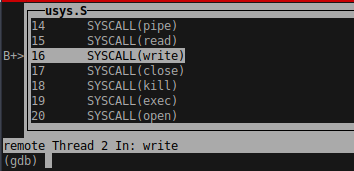
\includegraphics[width=\linewidth-8cm]{layoutsrc.png}
	\end{figure}
	\begin{figure}[H]
		\centering
		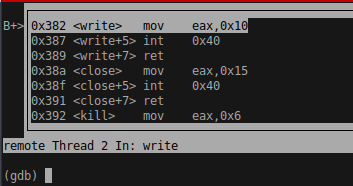
\includegraphics[width=\linewidth-8cm]{layoutasm.png}
	\end{figure}
	
	خروجی دستور 
	\lr{\lstinline|layout src|} 
	خطی از فایل 
	\lr{usys.S} 
	را نشان می‌دهد که منجر به فراخوانی سیستمی 
	\lr{\lstinline|write|} 
	می‌شود.
	
	خروجی دستور 
	\lr{\lstinline|layout asm|} 
	معادل اسمبلی این فرا‌خوانی است. برای فراخوانی سیستمی ابتدا باید شماره‌ی فراخوانی مورد نظر را در ثبات 
	\lr{eax} 
	بریزیم. شماره‌ی فراخوانی‌های سیستمی در سیستم‌ عامل لینوکس در آدرس 
	\lr{/usr/include/x86\_64-linux-gnu/asm/unistd\_64.h} 
	قرار دارند. بعد از این کار باید دستور 
	\lr{\lstinline|syscall|} 
	صدا زده شود که این کار با وقفه‌ی شماره 
	\lr{0x40} 
	صورت گرفته است. در نهایت برای برگشت از تایع کمکی 
	\lr{\lstinline|write|} 
	به فریم تابع 
	\lr{\lstinline|cat|} 
	از دستور 
	\lr{\lstinline|ret|} 
	استفاده شده است.
	قبل از فراخوانی 
	\lr{\lstinline|write|} 
	آرگومان‌های ورودی آن در پشته قرار دارند. این مدل از فراخوانی توابع در سیستم عامل‌های ۳۲ بیتی رواج دارد. در سیستم عامل‌های ۶۴ بیتی چند آرگومان اول نیز همانند شماره‌ی فراخوانی سیستمی در ثبات‌ها قرار ریخته می‌شوند. دستور 
	\lr{\lstinline|ret|} 
	به آدرسی که در سر پشته قرار دارد، برمی‌گردد. این آدرس توسط دستور 
	\lr{\lstinline|call|} 
	در پشته نوشته می‌شود.
\end{itemize}
\end{document}